\section{Transformer}

\subsection{Output}
\begin{frame}[c]{Output}
    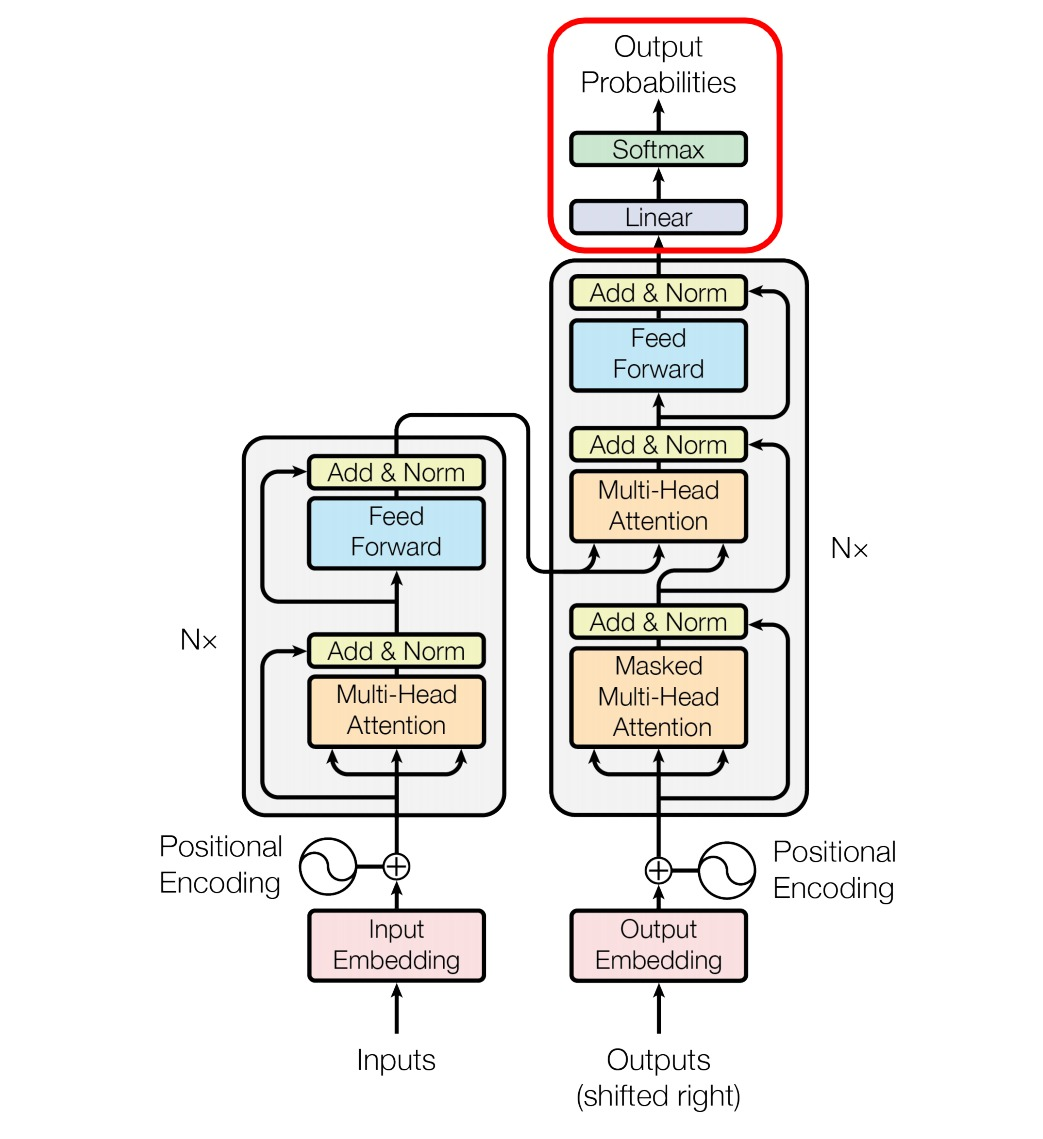
\includegraphics[height=0.9\textheight]{transformer_output}
    \pnote{
    followed by topk selection
    }
\end{frame}


\subsection{Dimensions}
\begin{frame}[c]{Dimensions} 
    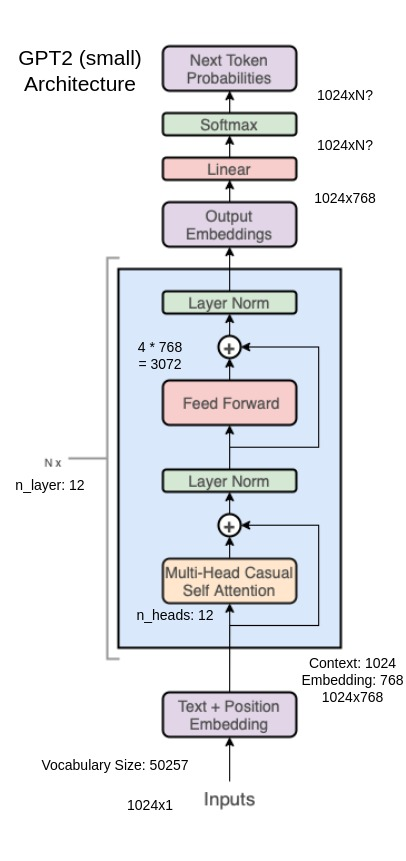
\includegraphics[height=\textheight]{gpt2_decoder_dims}
    \pnote{
        Dimensions represent my current understanding, reality might differ
    }
\end{frame}

\begin{frame}[c]{Dimensions II}
    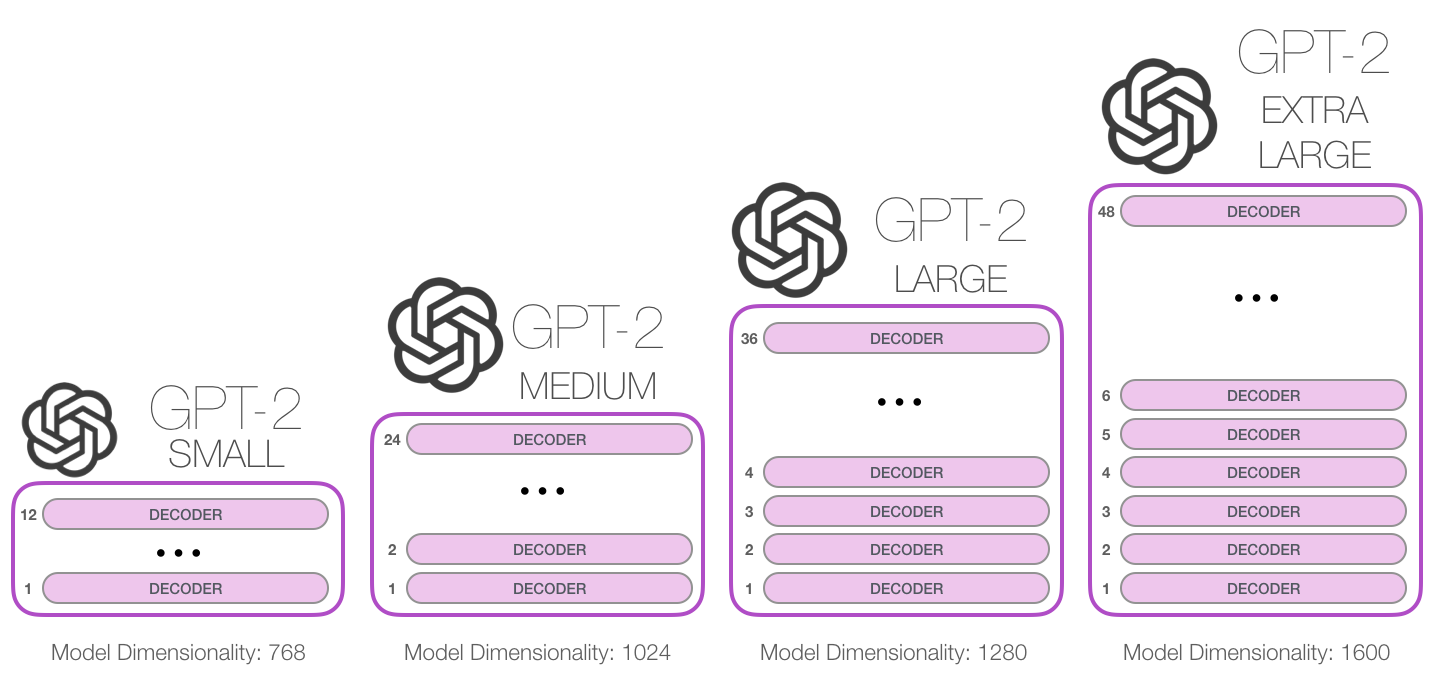
\includegraphics[width=\textwidth]{gpt2-sizes} \\
    Image Source: \cite{alammar_illustrated_2019}
\end{frame}


\subsection{Putting it all Together}
\begin{frame}[c]
    Full Architecture Overview
\end{frame}

\subsection{Interpretation}
\begin{frame}[c]
    Solving PDE \cite{lu_understanding_2019}
\end{frame}

\subsection{Sparse Transformer}
\begin{frame}[c]
    Even the original GPT didn't use 'full' transformers, but Sparse Transformer \cite{child_generating_2019}
\end{frame}

\subsection{Linear Time Transformers}
\begin{frame}[c]
    FastFormer \cite{wu_fastformer_2021} \\
    Transformer Quality in Linear Time \cite{hua_transformer_2022} \\
    FlashAttention \cite{dao_flashattention_2022}
\end{frame}

